\documentclass[]{book}
\usepackage{lmodern}
\usepackage{amssymb,amsmath}
\usepackage{ifxetex,ifluatex}
\usepackage{fixltx2e} % provides \textsubscript
\ifnum 0\ifxetex 1\fi\ifluatex 1\fi=0 % if pdftex
  \usepackage[T1]{fontenc}
  \usepackage[utf8]{inputenc}
\else % if luatex or xelatex
  \ifxetex
    \usepackage{mathspec}
  \else
    \usepackage{fontspec}
  \fi
  \defaultfontfeatures{Ligatures=TeX,Scale=MatchLowercase}
\fi
% use upquote if available, for straight quotes in verbatim environments
\IfFileExists{upquote.sty}{\usepackage{upquote}}{}
% use microtype if available
\IfFileExists{microtype.sty}{%
\usepackage{microtype}
\UseMicrotypeSet[protrusion]{basicmath} % disable protrusion for tt fonts
}{}
\usepackage[margin=1in]{geometry}
\usepackage{hyperref}
\hypersetup{unicode=true,
            pdftitle={ggplot2逆引き集},
            pdfauthor={@kazutan},
            pdfborder={0 0 0},
            breaklinks=true}
\urlstyle{same}  % don't use monospace font for urls
\usepackage{color}
\usepackage{fancyvrb}
\newcommand{\VerbBar}{|}
\newcommand{\VERB}{\Verb[commandchars=\\\{\}]}
\DefineVerbatimEnvironment{Highlighting}{Verbatim}{commandchars=\\\{\}}
% Add ',fontsize=\small' for more characters per line
\usepackage{framed}
\definecolor{shadecolor}{RGB}{248,248,248}
\newenvironment{Shaded}{\begin{snugshade}}{\end{snugshade}}
\newcommand{\KeywordTok}[1]{\textcolor[rgb]{0.13,0.29,0.53}{\textbf{{#1}}}}
\newcommand{\DataTypeTok}[1]{\textcolor[rgb]{0.13,0.29,0.53}{{#1}}}
\newcommand{\DecValTok}[1]{\textcolor[rgb]{0.00,0.00,0.81}{{#1}}}
\newcommand{\BaseNTok}[1]{\textcolor[rgb]{0.00,0.00,0.81}{{#1}}}
\newcommand{\FloatTok}[1]{\textcolor[rgb]{0.00,0.00,0.81}{{#1}}}
\newcommand{\ConstantTok}[1]{\textcolor[rgb]{0.00,0.00,0.00}{{#1}}}
\newcommand{\CharTok}[1]{\textcolor[rgb]{0.31,0.60,0.02}{{#1}}}
\newcommand{\SpecialCharTok}[1]{\textcolor[rgb]{0.00,0.00,0.00}{{#1}}}
\newcommand{\StringTok}[1]{\textcolor[rgb]{0.31,0.60,0.02}{{#1}}}
\newcommand{\VerbatimStringTok}[1]{\textcolor[rgb]{0.31,0.60,0.02}{{#1}}}
\newcommand{\SpecialStringTok}[1]{\textcolor[rgb]{0.31,0.60,0.02}{{#1}}}
\newcommand{\ImportTok}[1]{{#1}}
\newcommand{\CommentTok}[1]{\textcolor[rgb]{0.56,0.35,0.01}{\textit{{#1}}}}
\newcommand{\DocumentationTok}[1]{\textcolor[rgb]{0.56,0.35,0.01}{\textbf{\textit{{#1}}}}}
\newcommand{\AnnotationTok}[1]{\textcolor[rgb]{0.56,0.35,0.01}{\textbf{\textit{{#1}}}}}
\newcommand{\CommentVarTok}[1]{\textcolor[rgb]{0.56,0.35,0.01}{\textbf{\textit{{#1}}}}}
\newcommand{\OtherTok}[1]{\textcolor[rgb]{0.56,0.35,0.01}{{#1}}}
\newcommand{\FunctionTok}[1]{\textcolor[rgb]{0.00,0.00,0.00}{{#1}}}
\newcommand{\VariableTok}[1]{\textcolor[rgb]{0.00,0.00,0.00}{{#1}}}
\newcommand{\ControlFlowTok}[1]{\textcolor[rgb]{0.13,0.29,0.53}{\textbf{{#1}}}}
\newcommand{\OperatorTok}[1]{\textcolor[rgb]{0.81,0.36,0.00}{\textbf{{#1}}}}
\newcommand{\BuiltInTok}[1]{{#1}}
\newcommand{\ExtensionTok}[1]{{#1}}
\newcommand{\PreprocessorTok}[1]{\textcolor[rgb]{0.56,0.35,0.01}{\textit{{#1}}}}
\newcommand{\AttributeTok}[1]{\textcolor[rgb]{0.77,0.63,0.00}{{#1}}}
\newcommand{\RegionMarkerTok}[1]{{#1}}
\newcommand{\InformationTok}[1]{\textcolor[rgb]{0.56,0.35,0.01}{\textbf{\textit{{#1}}}}}
\newcommand{\WarningTok}[1]{\textcolor[rgb]{0.56,0.35,0.01}{\textbf{\textit{{#1}}}}}
\newcommand{\AlertTok}[1]{\textcolor[rgb]{0.94,0.16,0.16}{{#1}}}
\newcommand{\ErrorTok}[1]{\textcolor[rgb]{0.64,0.00,0.00}{\textbf{{#1}}}}
\newcommand{\NormalTok}[1]{{#1}}
\usepackage{longtable,booktabs}
\usepackage{graphicx,grffile}
\makeatletter
\def\maxwidth{\ifdim\Gin@nat@width>\linewidth\linewidth\else\Gin@nat@width\fi}
\def\maxheight{\ifdim\Gin@nat@height>\textheight\textheight\else\Gin@nat@height\fi}
\makeatother
% Scale images if necessary, so that they will not overflow the page
% margins by default, and it is still possible to overwrite the defaults
% using explicit options in \includegraphics[width, height, ...]{}
\setkeys{Gin}{width=\maxwidth,height=\maxheight,keepaspectratio}
\IfFileExists{parskip.sty}{%
\usepackage{parskip}
}{% else
\setlength{\parindent}{0pt}
\setlength{\parskip}{6pt plus 2pt minus 1pt}
}
\setlength{\emergencystretch}{3em}  % prevent overfull lines
\providecommand{\tightlist}{%
  \setlength{\itemsep}{0pt}\setlength{\parskip}{0pt}}
\setcounter{secnumdepth}{5}
% Redefines (sub)paragraphs to behave more like sections
\ifx\paragraph\undefined\else
\let\oldparagraph\paragraph
\renewcommand{\paragraph}[1]{\oldparagraph{#1}\mbox{}}
\fi
\ifx\subparagraph\undefined\else
\let\oldsubparagraph\subparagraph
\renewcommand{\subparagraph}[1]{\oldsubparagraph{#1}\mbox{}}
\fi

%%% Use protect on footnotes to avoid problems with footnotes in titles
\let\rmarkdownfootnote\footnote%
\def\footnote{\protect\rmarkdownfootnote}

%%% Change title format to be more compact
\usepackage{titling}

% Create subtitle command for use in maketitle
\newcommand{\subtitle}[1]{
  \posttitle{
    \begin{center}\large#1\end{center}
    }
}

\setlength{\droptitle}{-2em}
  \title{ggplot2逆引き集}
  \pretitle{\vspace{\droptitle}\centering\huge}
  \posttitle{\par}
  \author{@kazutan}
  \preauthor{\centering\large\emph}
  \postauthor{\par}
  \predate{\centering\large\emph}
  \postdate{\par}
  \date{2016-11-12}

\usepackage{luatexja}
\usepackage{luatexja-fontspec}
\setmainjfont{IPAGothic}
\setsansjfont{IPAGothic}

\begin{document}
\maketitle

{
\setcounter{tocdepth}{1}
\tableofcontents
}
これはQiitaで公開されている\textbf{ggplot2逆引き}の記事を集めたものです。

またこれは\texttt{bookdown}パッケージのテストを兼ねています。うまく動くといいなぁ\ldots{}。

\chapter{ggplot2で同一グラフに2変数の折れ線グラフを描きたい}\label{ggplot22}

\section{Q}\label{q}

このようなデータが手元にあります:

\begin{Shaded}
\begin{Highlighting}[]
\NormalTok{test_data <-}\StringTok{ }\KeywordTok{data.frame}\NormalTok{(}
\DataTypeTok{var0 =} \DecValTok{100} \NormalTok{+}\StringTok{ }\KeywordTok{c}\NormalTok{(}\DecValTok{0}\NormalTok{, }\KeywordTok{cumsum}\NormalTok{(}\KeywordTok{runif}\NormalTok{(}\DecValTok{49}\NormalTok{, -}\DecValTok{20}\NormalTok{, }\DecValTok{20}\NormalTok{))),}
\DataTypeTok{var1 =} \DecValTok{150} \NormalTok{+}\StringTok{ }\KeywordTok{c}\NormalTok{(}\DecValTok{0}\NormalTok{, }\KeywordTok{cumsum}\NormalTok{(}\KeywordTok{runif}\NormalTok{(}\DecValTok{49}\NormalTok{, -}\DecValTok{10}\NormalTok{, }\DecValTok{10}\NormalTok{))),}
\DataTypeTok{date =} \KeywordTok{seq.Date}\NormalTok{(}\KeywordTok{as.Date}\NormalTok{(}\StringTok{"2002-01-01"}\NormalTok{), }\DataTypeTok{by=}\StringTok{"1 month"}\NormalTok{, }\DataTypeTok{length.out=}\DecValTok{100}\NormalTok{))}
\end{Highlighting}
\end{Shaded}

この時系列変数\texttt{var0}と\texttt{var1}の両方共を、\texttt{date}をx軸にして\texttt{ggplot2}でどうやったら描けますか?
できれば\texttt{var0}と\texttt{var1}の色を変えて、さらに凡例も付けれたら嬉しいです。

\section{A}\label{a}

もし変数が少ないのであれば、マニュアルで別々に作成ビルドアップできますよ:

\begin{Shaded}
\begin{Highlighting}[]
\KeywordTok{library}\NormalTok{(ggplot2)}
\KeywordTok{ggplot}\NormalTok{(test_data, }\KeywordTok{aes}\NormalTok{(date)) +}
\StringTok{  }\KeywordTok{geom_line}\NormalTok{(}\KeywordTok{aes}\NormalTok{(}\DataTypeTok{y =} \NormalTok{var0, }\DataTypeTok{colour =} \StringTok{"var0"}\NormalTok{)) +}
\StringTok{  }\KeywordTok{geom_line}\NormalTok{(}\KeywordTok{aes}\NormalTok{(}\DataTypeTok{y =} \NormalTok{var1, }\DataTypeTok{colour =} \StringTok{"var1"}\NormalTok{))}
\end{Highlighting}
\end{Shaded}

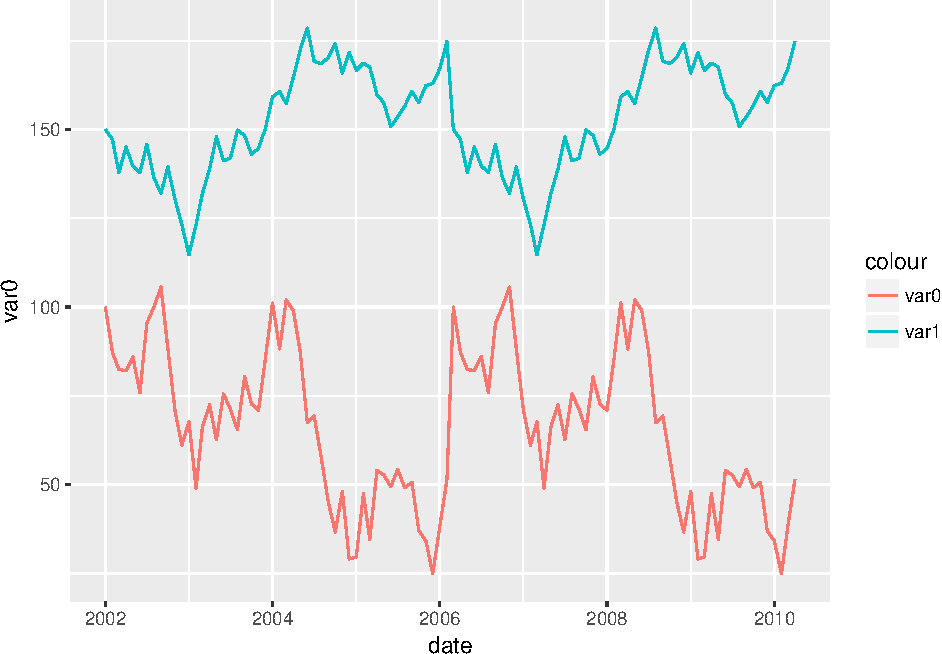
\includegraphics{ggplot2-gyakubiki-book_files/figure-latex/unnamed-chunk-2-1.pdf}

一般的なアプローチとしては、\texttt{tydyr}パッケージを利用してデータを縦型(long
format)に変換していく方法があります:

\begin{Shaded}
\begin{Highlighting}[]
\KeywordTok{library}\NormalTok{(tidyr)}
\KeywordTok{library}\NormalTok{(ggplot2)}

\NormalTok{test_data_long <-}\StringTok{ }\NormalTok{tidyr::}\KeywordTok{gather}\NormalTok{(test_data, }\DataTypeTok{key=}\StringTok{"variable"}\NormalTok{, }\DataTypeTok{value =} \NormalTok{value, -date) }\CommentTok{# 縦型に変換}

\NormalTok{knitr::}\KeywordTok{kable}\NormalTok{(}\KeywordTok{head}\NormalTok{(test_data_long, }\DecValTok{6}\NormalTok{))}
\end{Highlighting}
\end{Shaded}

\begin{tabular}{l|l|r}
\hline
date & variable & value\\
\hline
2002-01-01 & var0 & 100.00000\\
\hline
2002-02-01 & var0 & 87.20176\\
\hline
2002-03-01 & var0 & 82.41162\\
\hline
2002-04-01 & var0 & 82.10215\\
\hline
2002-05-01 & var0 & 86.00951\\
\hline
2002-06-01 & var0 & 75.88203\\
\hline
\end{tabular}

\begin{Shaded}
\begin{Highlighting}[]
\KeywordTok{ggplot}\NormalTok{(}\DataTypeTok{data=}\NormalTok{test_data_long, }\KeywordTok{aes}\NormalTok{(}\DataTypeTok{x=}\NormalTok{date, }\DataTypeTok{y=}\NormalTok{value, }\DataTypeTok{colour=}\NormalTok{variable)) +}
\StringTok{  }\KeywordTok{geom_line}\NormalTok{()}
\end{Highlighting}
\end{Shaded}

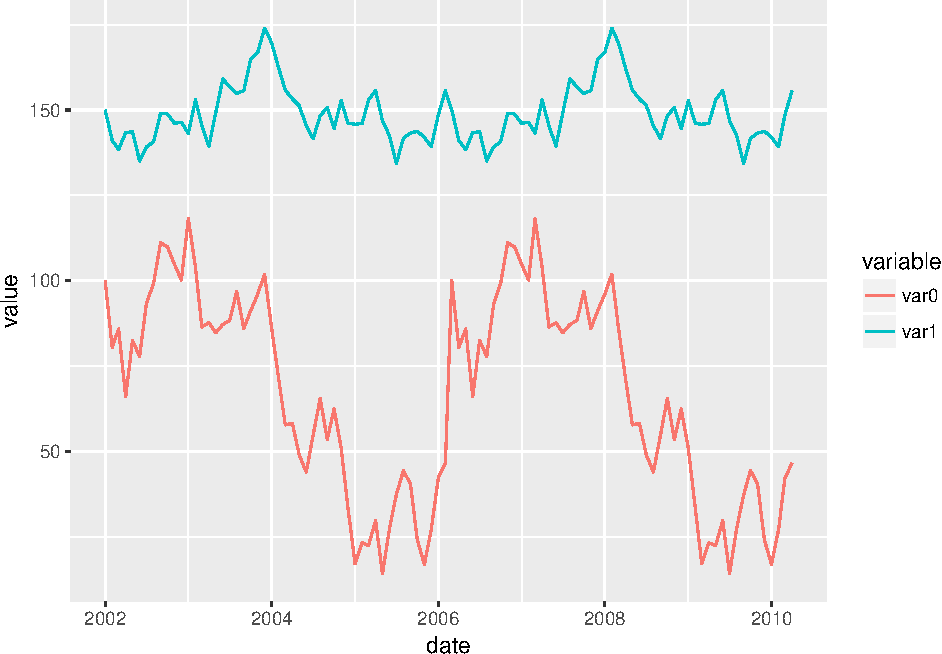
\includegraphics{ggplot2-gyakubiki-book_files/figure-latex/unnamed-chunk-3-1.pdf}

データを縦型のデータに変換し、\texttt{var0}と\texttt{var1}を分けるための変数で色分けを指定すればこのようになります。

\section{参考}

この記事は、StackOverflowに投稿された以下の記事をベースに、コードを一部改変して翻訳して作成しました:
-
\href{http://stackoverflow.com/questions/3777174/plotting-two-variables-as-lines-using-ggplot2-on-the-same-graph}{r
- Plotting two variables as lines using ggplot2 on the same graph -
Stack Overflow}

関連ドキュメント: -
\href{http://docs.ggplot2.org/current/geom_line.html}{geom\_line.
ggplot2 0.9.3.1}

\chapter{ggplot2で積み重ね棒グラフに値を表示させたい}\label{ggplot2}

\textbf{2016/04/12追記: ggplot2
v2.1.0に対応するため、一部コードを修正しました}

\begin{quote}
本記事は
\href{http://qiita.com/tags/ggplot2\%E9\%80\%86\%E5\%BC\%95\%E3\%81\%8D/items}{ggplot2逆引き}
プロジェクトの一環として、Stack Oveflow の下記記事を翻訳したものです。\\
\href{http://stackoverflow.com/questions/6644997/showing-data-values-on-stacked-bar-chart-in-ggplot2}{r
- Showing data values on stacked bar chart in ggplot2 - Stack Overflow}
\end{quote}

\section{Q}\label{q-1}

ggplot2で積み重ね棒グラフに値を重ねて表示したいです。私が試したのは以下のコードです:

\textbf{2016/04/12追記: ggplot2
v2.1.0で\texttt{qplot()}の仕様が変更されているようでしたので、\texttt{ggplot()}で描くように修正しました}

\begin{Shaded}
\begin{Highlighting}[]
\NormalTok{Year      <-}\StringTok{ }\KeywordTok{c}\NormalTok{(}\KeywordTok{rep}\NormalTok{(}\KeywordTok{c}\NormalTok{(}\StringTok{"2006-07"}\NormalTok{, }\StringTok{"2007-08"}\NormalTok{, }\StringTok{"2008-09"}\NormalTok{, }\StringTok{"2009-10"}\NormalTok{), }\DataTypeTok{each =} \DecValTok{4}\NormalTok{))}
\NormalTok{Category  <-}\StringTok{ }\KeywordTok{c}\NormalTok{(}\KeywordTok{rep}\NormalTok{(}\KeywordTok{c}\NormalTok{(}\StringTok{"A"}\NormalTok{, }\StringTok{"B"}\NormalTok{, }\StringTok{"C"}\NormalTok{, }\StringTok{"D"}\NormalTok{), }\DataTypeTok{times =} \DecValTok{4}\NormalTok{))}
\NormalTok{Frequency <-}\StringTok{ }\KeywordTok{c}\NormalTok{(}\DecValTok{168}\NormalTok{, }\DecValTok{259}\NormalTok{, }\DecValTok{226}\NormalTok{, }\DecValTok{340}\NormalTok{, }\DecValTok{216}\NormalTok{, }\DecValTok{431}\NormalTok{, }\DecValTok{319}\NormalTok{, }\DecValTok{368}\NormalTok{, }\DecValTok{423}\NormalTok{, }\DecValTok{645}\NormalTok{, }\DecValTok{234}\NormalTok{, }\DecValTok{685}\NormalTok{, }\DecValTok{166}\NormalTok{, }\DecValTok{467}\NormalTok{, }\DecValTok{274}\NormalTok{, }\DecValTok{251}\NormalTok{)}
\NormalTok{Data      <-}\StringTok{ }\KeywordTok{data.frame}\NormalTok{(Year, Category, Frequency)}
\KeywordTok{library}\NormalTok{(ggplot2)}
\NormalTok{p <-}\StringTok{ }\KeywordTok{ggplot}\NormalTok{(Data, }\KeywordTok{aes}\NormalTok{(Year, Frequency, }\DataTypeTok{fill =} \NormalTok{Category)) +}
\StringTok{  }\KeywordTok{geom_bar}\NormalTok{(}\DataTypeTok{stat =} \StringTok{"identity"}\NormalTok{) +}
\StringTok{  }\KeywordTok{theme_bw}\NormalTok{()}
\NormalTok{p +}\StringTok{ }\KeywordTok{geom_text}\NormalTok{(}\KeywordTok{aes}\NormalTok{(}\DataTypeTok{label =} \NormalTok{Frequency), }\DataTypeTok{size =} \DecValTok{3}\NormalTok{, }\DataTypeTok{hjust =} \FloatTok{0.5}\NormalTok{, }\DataTypeTok{vjust =} \DecValTok{3}\NormalTok{, }\DataTypeTok{position =} \StringTok{"stack"}\NormalTok{) }
\end{Highlighting}
\end{Shaded}

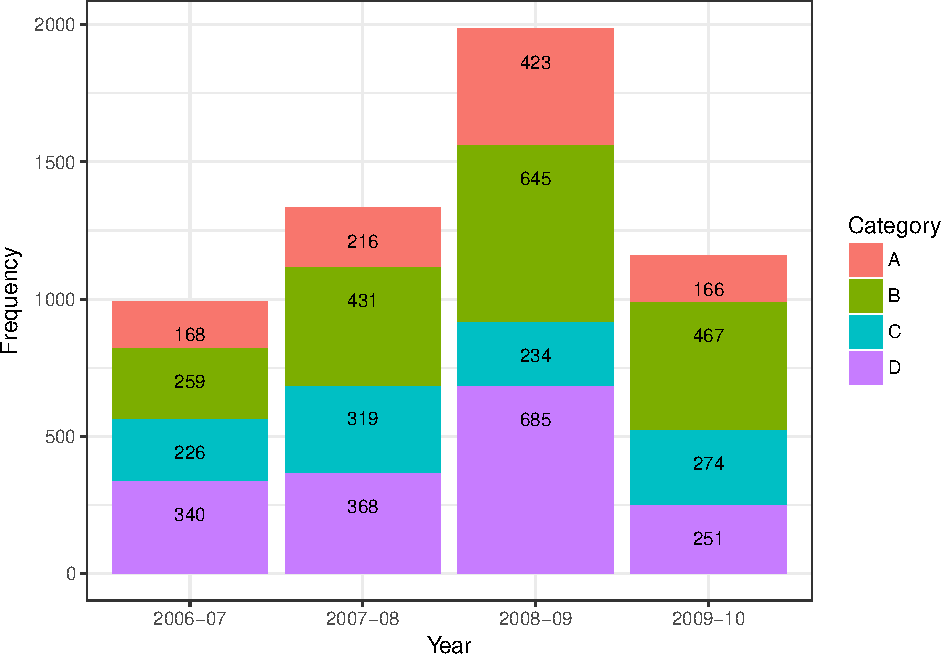
\includegraphics{ggplot2-gyakubiki-book_files/figure-latex/unnamed-chunk-4-1.pdf}

でもこのデータの値を、各部位の中央に配置したいのです。お願いします。

\section{A}\label{a-1}

一つのやり方として、各バーのミッドポイントを算出するというのがあります:

\begin{Shaded}
\begin{Highlighting}[]
\KeywordTok{library}\NormalTok{(plyr)}
\KeywordTok{library}\NormalTok{(ggplot2)}

\CommentTok{# calculate midpoints of bars (simplified using comment by @DWin)}
\NormalTok{Data <-}\StringTok{ }\KeywordTok{ddply}\NormalTok{(Data, .(Year), transform, }\DataTypeTok{pos =} \KeywordTok{cumsum}\NormalTok{(Frequency) -}\StringTok{ }\NormalTok{(}\FloatTok{0.5} \NormalTok{*}\StringTok{ }\NormalTok{Frequency))}

\CommentTok{# plot bars and add text}
\NormalTok{p <-}\StringTok{ }\KeywordTok{ggplot}\NormalTok{(Data, }\KeywordTok{aes}\NormalTok{(}\DataTypeTok{x =} \NormalTok{Year, }\DataTypeTok{y =} \NormalTok{Frequency)) +}
\StringTok{     }\KeywordTok{geom_bar}\NormalTok{(}\KeywordTok{aes}\NormalTok{(}\DataTypeTok{fill =} \NormalTok{Category), }\DataTypeTok{stat=}\StringTok{"identity"}\NormalTok{) +}
\StringTok{     }\KeywordTok{geom_text}\NormalTok{(}\KeywordTok{aes}\NormalTok{(}\DataTypeTok{label =} \NormalTok{Frequency, }\DataTypeTok{y =} \NormalTok{pos), }\DataTypeTok{size =} \DecValTok{3}\NormalTok{)}
\end{Highlighting}
\end{Shaded}

\begin{Shaded}
\begin{Highlighting}[]
\KeywordTok{library}\NormalTok{(plyr)}
\KeywordTok{library}\NormalTok{(ggplot2)}
\NormalTok{Year      <-}\StringTok{ }\KeywordTok{c}\NormalTok{(}\KeywordTok{rep}\NormalTok{(}\KeywordTok{c}\NormalTok{(}\StringTok{"2006-07"}\NormalTok{, }\StringTok{"2007-08"}\NormalTok{, }\StringTok{"2008-09"}\NormalTok{, }\StringTok{"2009-10"}\NormalTok{), }\DataTypeTok{each =} \DecValTok{4}\NormalTok{))}
\NormalTok{Category  <-}\StringTok{ }\KeywordTok{c}\NormalTok{(}\KeywordTok{rep}\NormalTok{(}\KeywordTok{c}\NormalTok{(}\StringTok{"A"}\NormalTok{, }\StringTok{"B"}\NormalTok{, }\StringTok{"C"}\NormalTok{, }\StringTok{"D"}\NormalTok{), }\DataTypeTok{times =} \DecValTok{4}\NormalTok{))}
\NormalTok{Frequency <-}\StringTok{ }\KeywordTok{c}\NormalTok{(}\DecValTok{168}\NormalTok{, }\DecValTok{259}\NormalTok{, }\DecValTok{226}\NormalTok{, }\DecValTok{340}\NormalTok{, }\DecValTok{216}\NormalTok{, }\DecValTok{431}\NormalTok{, }\DecValTok{319}\NormalTok{, }\DecValTok{368}\NormalTok{, }\DecValTok{423}\NormalTok{, }\DecValTok{645}\NormalTok{, }\DecValTok{234}\NormalTok{, }\DecValTok{685}\NormalTok{, }\DecValTok{166}\NormalTok{, }\DecValTok{467}\NormalTok{, }\DecValTok{274}\NormalTok{, }\DecValTok{251}\NormalTok{)}
\NormalTok{Data      <-}\StringTok{ }\KeywordTok{data.frame}\NormalTok{(Year, Category, Frequency)}

\CommentTok{# calculate midpoints of bars (simplified using comment by @DWin)}
\NormalTok{Data <-}\StringTok{ }\KeywordTok{ddply}\NormalTok{(Data, .(Year), transform, }\DataTypeTok{pos =} \KeywordTok{cumsum}\NormalTok{(Frequency) -}\StringTok{ }\NormalTok{(}\FloatTok{0.5} \NormalTok{*}\StringTok{ }\NormalTok{Frequency))}

\CommentTok{# plot bars and add text}
\NormalTok{p <-}\StringTok{ }\KeywordTok{ggplot}\NormalTok{(Data, }\KeywordTok{aes}\NormalTok{(}\DataTypeTok{x =} \NormalTok{Year, }\DataTypeTok{y =} \NormalTok{Frequency)) +}
\StringTok{     }\KeywordTok{geom_bar}\NormalTok{(}\KeywordTok{aes}\NormalTok{(}\DataTypeTok{fill =} \NormalTok{Category), }\DataTypeTok{stat=}\StringTok{"identity"}\NormalTok{) +}
\StringTok{     }\KeywordTok{geom_text}\NormalTok{(}\KeywordTok{aes}\NormalTok{(}\DataTypeTok{label =} \NormalTok{Frequency, }\DataTypeTok{y =} \NormalTok{pos), }\DataTypeTok{size =} \DecValTok{3}\NormalTok{)}
\NormalTok{p}
\end{Highlighting}
\end{Shaded}

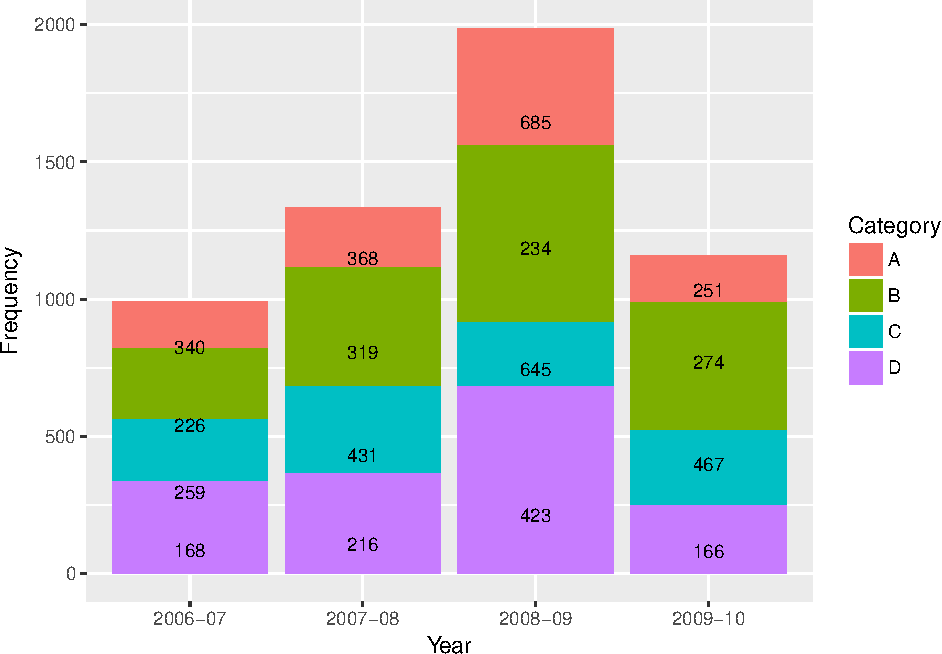
\includegraphics{ggplot2-gyakubiki-book_files/figure-latex/unnamed-chunk-6-1.pdf}

データフレームにあらかじめ値を配置する高さ(y値)を算出して変数として追加し、\texttt{geom\_text(aes(label\ =\ Frequency,\ y\ =\ pos))}とその変数を指定すれば、そのラベルは算出した位置に配置されます。

\section{補足}

上記のAの方法は、データフレームに新たに変数を追加することとなります。それを避けて(だいたい)真ん中にくるようになればいい、というのであれば、以下のようなコードでも可能です:

\begin{Shaded}
\begin{Highlighting}[]
\NormalTok{p <-}\StringTok{ }\KeywordTok{ggplot}\NormalTok{(Data, }\KeywordTok{aes}\NormalTok{(}\DataTypeTok{x =} \NormalTok{Year, }\DataTypeTok{y =} \NormalTok{Frequency)) +}
\StringTok{  }\KeywordTok{geom_bar}\NormalTok{(}\KeywordTok{aes}\NormalTok{(}\DataTypeTok{fill =} \NormalTok{Category), }\DataTypeTok{stat=}\StringTok{"identity"}\NormalTok{) +}
\StringTok{  }\KeywordTok{geom_text}\NormalTok{(}\KeywordTok{aes}\NormalTok{(}\DataTypeTok{label =} \NormalTok{Frequency), }\DataTypeTok{size =} \DecValTok{3}\NormalTok{, }\DataTypeTok{position =} \StringTok{"stack"}\NormalTok{, }\DataTypeTok{vjust =} \NormalTok{Frequency/}\DecValTok{75}\NormalTok{)}
\NormalTok{p}
\end{Highlighting}
\end{Shaded}

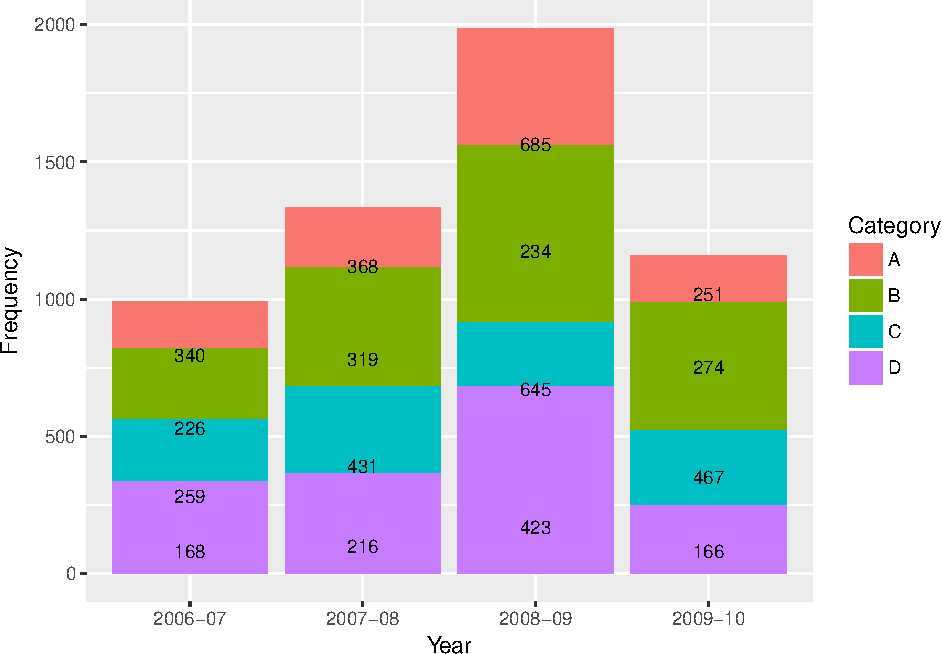
\includegraphics{ggplot2-gyakubiki-book_files/figure-latex/unnamed-chunk-7-1.pdf}

これは、\texttt{geom-text}の\texttt{vjust}に対して設定を加えています。このようにy値の変数を定数で補正したものを\texttt{vjust\ =}に投げると、割合的にずれてくれるようになります。

ただこの方法ですと、その補正する定数をどう設定したらど真ん中にくるか、はっきりとはわかりません。詳しくは\href{https://rpubs.com/kazutan/vjust_test}{RPubs
- vjustのテスト}をご覧ください。

また、この記事の元となっているStackOverflowの記事には、Hadley
Wickham氏による以下のコメントがあったことも付記します:

\begin{quote}
Please don't. It's not a good idea to try and improve a confusing
visualisation by adding text labels. Either make a table or use a better
display of the data. -- hadley Jul 12 '11 at 1:10
\end{quote}

\section{参考}\label{-1}

\begin{itemize}
\tightlist
\item
  \href{http://stackoverflow.com/questions/6644997/showing-data-values-on-stacked-bar-chart-in-ggplot2}{r
  - Showing data values on stacked bar chart in ggplot2 - Stack
  Overflow}
\item
  \href{https://rpubs.com/kazutan/vjust_test}{RPubs - vjustのテスト}
\item
  \href{http://qiita.com/hoxo_m/items/267ce2ab0acc319599ff}{ggplot2逆引き
  - ggplot2 で geom\_text() を使って集合棒グラフにラベルを付けたい
  \#rstatsj - Qiita}
\end{itemize}


\end{document}
